\subsection{Sample and variables}

We use two mature British cohort studies that have been widely used by economists and sociologists to examine the extent of mobility in the UK. The National Child Development Study (NCDS58) is a cohort of individuals born during a given week in March 1958. The British Cohort Study (BCS70) is composed of individuals born during a given week in April 1970. Cohort members were born in England, Scotland, Wales and Northern Ireland and participated in several interviews at different points in time over their life. 
\begin{figure}[!tb]
    \centering
    \caption{Dates of interviews}
    \label{chap2-fig:interviews}
    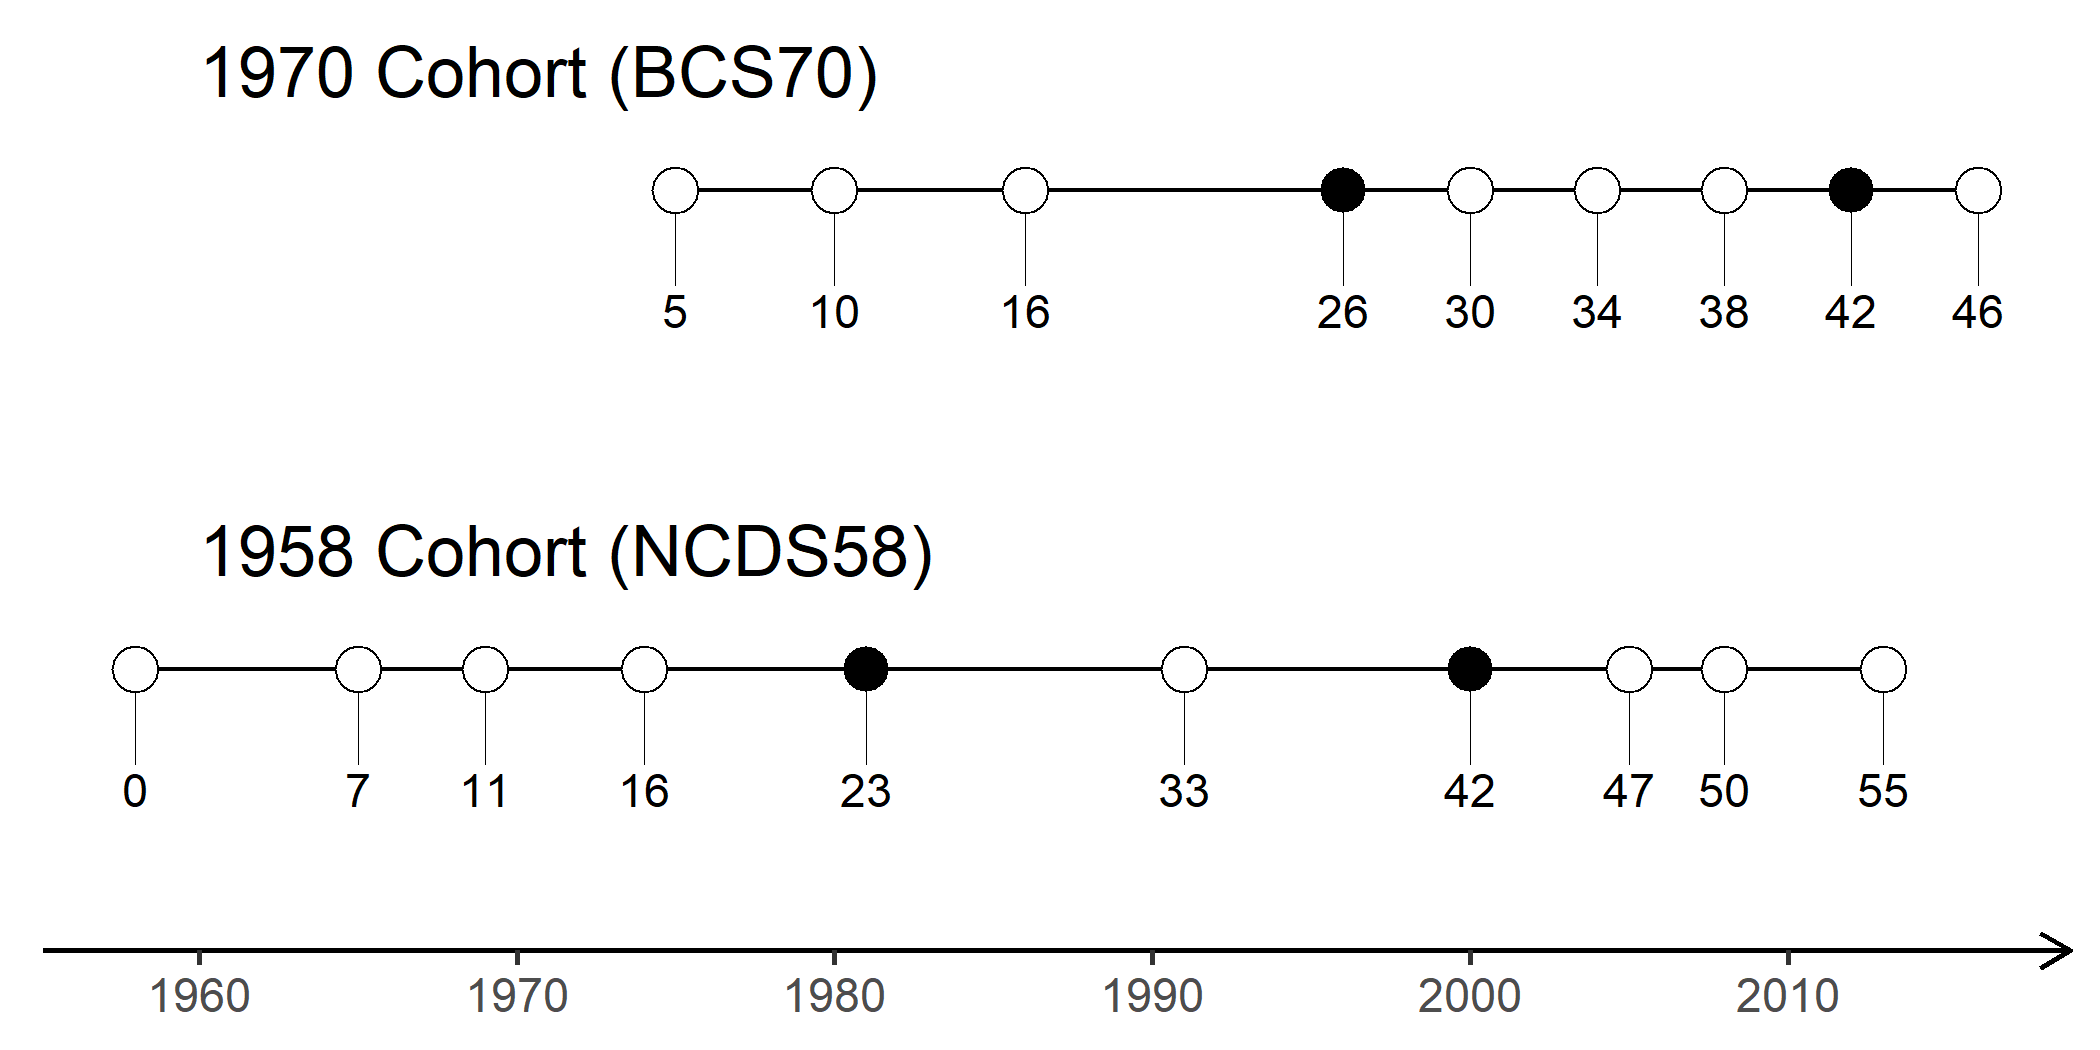
\includegraphics[width=\linewidth]{chap2/graphic/itw-date-spreadpol.png}
	\vspace{-3em}
	\justify\singlespacing\footnotesize{\textit{Notes:} This figure presents the dates at which individuals in the BCS70 and NCDS58 cohorts may have been interviewed and the corresponding years. Black circles represent the first and second periods we consider in the analysis for both cohorts.}
\end{figure}
Figure \ref{chap2-fig:interviews} presents all the interviews at which cohort members were interviewed and the corresponding year.

\textbf{Periods.} We define the first period as the year of interview closest to that in which the individual was 25 years-old, the age usually considered as that of entry into the labour market. Those in the NCDS58 cohort are observed at age 23 and those in the BCS70 cohort at age 26. Both cohorts are interviewed at age 42, which we define as the second period.

\textbf{Income and wages.} We have information on parental income, which is provided when the child was 16 years-old for both cohorts. For the BCS70 cohort, it is also available when the child was 10. Thus, when both are available, we take the average of the two observations; otherwise we use the single one we observe.\footnote{\cite{Blanden2013Intergenerational} show that the observed increase in the role of parental income to determine child's income is not driven by the poor measurement of permanent income in the 1958 cohort.} In order to adjust both for inflation, aggregate income growth and changes in the dispersion of income, parental income is standardized, so that for both cohorts it has mean zero and a variance of 1 (see Table \ref{chap2-tab:stat-indiv} for the summary statistics).

For children, we observe wages, which are reported at each wave. We adjust for inflation using the consumer price index provided by the \href{https://www.ons.gov.uk/economy/inflationandpriceindices}{UK Office for National Statistics}. The resulting monetary variables are all expressed in 1970 British pounds. 

% International Standard Classification of Occupations 1988 (ISCO-88)
\textbf{Occupational categories.} Both cohorts studies provide the full activity histories to the nearest month from which we can derive the ISCO-88 occupations.\footnote{Cohort data provide 3-digit occupations in the \href{https://www.hesa.ac.uk/support/documentation/occupational/soc90}{Standard Occupational Classification 1990 (SOC90)} and the \href{https://www.hesa.ac.uk/support/documentation/occupational/soc2000}{Standard Occupational Classification 2000 (SOC2000)}. We can derive ISCO-88 occupations by using the files from \href{http://www.camsis.stir.ac.uk/occunits/distribution.html}{CAMSIS project} which cover both SOC occupational unit codes and translations into ISCO-88.}
We aggregate ISCO-88 occupations into three categories: high-paying, middling and low-paying occupations. This classification follows the job-polarization literature and is consistent with that used in \cite{Goos2014Explaining} and \cite{Mahutga2018Job}.\footnote{A large body of literature on social mobility relies on the National Statistics Socio-Economic Classification (NS-SEC), starting with \cite{Erikson1992Constant} and \cite{Rose1998ESRC}. However, such classification uses a definition of routine occupations that does not match that used in the job-polarization literature. For instance, the NS-SEC considers that an employee in the 3-digit occupation \textit{Bar staff (622)} has a routine occupation. However, it cannot be considered as a routine job following the definition of \cite{Autor2003Skill} who define this type of job as a non-routine interactive job. We hence chose not to rely on the NS-SEC for our analysis.} Table \ref{chap2-tab:data-isco88} in the appendix presents the classification.  For completeness, we also include a fourth category---individuals who are out-of-work. This category groups those out of the labour force, those who are unemployed, and those in full-time study. Table \ref{chap2-tab:stat-cohper} displays the shares of the various activity status and occupational categories in the cohort data.

As has been shown in previous work, occupational categories are closely related to remuneration levels, and we document this for our cohort data in the appendix. Table \ref{chap2-tab:stat-pay} reports the average weekly pay by occupation, and displays the expected correlation between occupations and pay. 

\textbf{Location.} Since individuals give their address at each interview, we also have their location history. We focus on the region of residence at the age of 16 because it is the age at which the parental income variable is defined. The classification is prior to 1994 and thus uses the Government Offices for the Regions (GORs). We therefore rely on the Standard Statistical Regions (SSR).\footnote{For England, this is the highest sub-national division, while the other countries in Britain consists of a single region. The regions are (in alphabetical order): East Anglia, East Midlands, North, North West, Scotland, South East, South West, Wales, West Midlands, and Yorkshire and Humberside.} Table \ref{chap2-tab:stat-location} reports the share of cohort members in each region for both periods.

Once we restrict the data to those individuals for whom we have the key characteristics, i.e. parental income and occupations, our sample consists of 6,780 individuals in the NCDS58 and 7,983 in the BCS70, as reported in Table \ref{chap2-tab:stat-indiv}.

\textbf{The Labour Force Survey.} As a complementary dataset we use the Labor Force Survey (LFS). The LFS provides data on both labour market status and region of residence. It has the advantage of containing a much larger number of observations (see Appendix \ref{chap2-app-data-LFS} for the details), and allows us to compare the changes in the occupational structure in the cohort data with those from a larger sample, as well as to compute measures of polarization at the regional level.


\subsection{The structure of employment}

% Contribution - alternative view of polarization to the usual snapshot
Before proceeding to our empirical analysis, we consider the extent to which the two cohorts experienced different degrees of polarization. We start by looking at the change in the distribution of occupations at ages 23/26 and 42 for both cohorts, reported in Figure \ref{chap2-fig:stat-occ}.\footnote{We report the proportion of individuals in each occupation for the two cohorts in Tables \ref{chap2-tab:proba-group4-abs} and \ref{chap2-tab:proba-group5-abs} in the appendix.} In the first period there is an increase across cohorts in the probability of working in a high- and low-paying occupation and a decline in that of working in a middling-paying occupation. When we consider the occupations at age 42, the changes are of smaller magnitude, and the main difference across the two cohorts is a reduction in the share of middling jobs that has been offset by high-paying ones. These changes are consistent with the literature on polarization in the UK that shows a considerable decline in middling jobs, and an increase in the other two categories, which is particularly large for high-paying jobs (see Figure \ref{chap2-fig:lfs-national} in the appendix). The differences between the first and second period distributions are interesting for our purposes, as they raise the question of whether polarization in the first period matters even when the changes in the distribution of employment are small for mature individuals. 
\begin{figure}[!tb]
    \centering
    \caption{Occupation distribution across cohorts}
    \label{chap2-fig:stat-occ}
    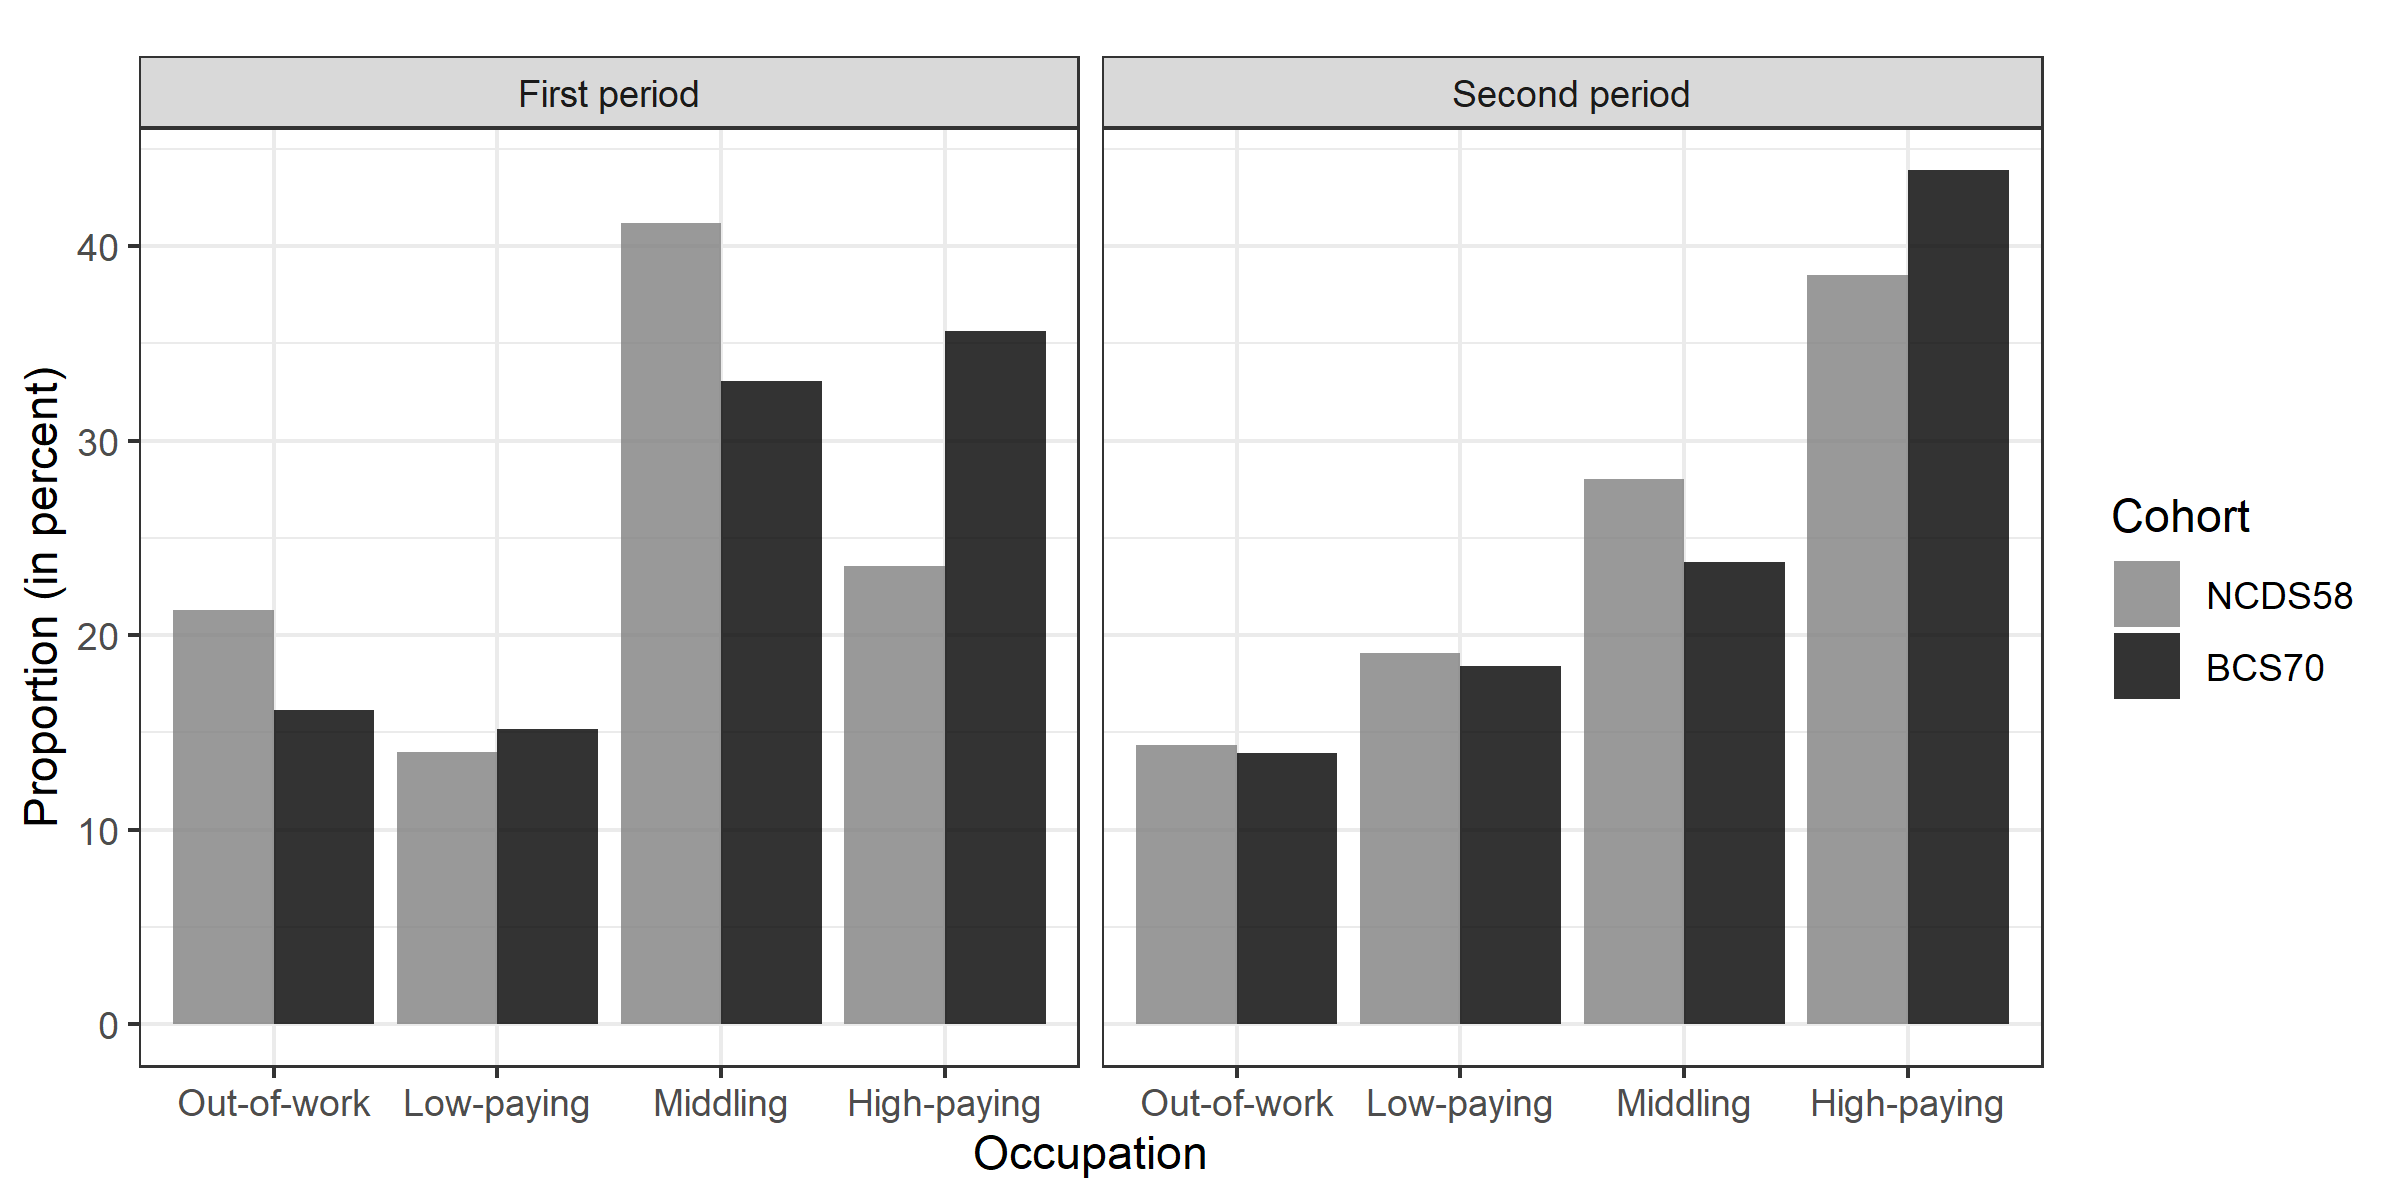
\includegraphics[width=\linewidth]{chap2/graphic/stat-occ.png}
	\vspace{-3em}
	\justify\singlespacing\footnotesize{\textit{Notes:} This figure reports the proportion of individuals, expressed in percent, in each type of occupation (out-of-work, low-paying, middling, high-paying) for the NCDS58 and BCS70 cohorts according to the period.}
\end{figure}
To better understand these dynamics, Figure \ref{chap2-fig:polarize-isco88-both} in the Appendix performs a similar exercise using the ISCO-88 categories, and shows a clear pattern of polarization, which has been particularly large for young individual.

As an alternative way of thinking about polarization we examine how occupations with either different average pay or  ``routine task intensity'' (RTI) have changed across the two cohorts, reported in Figure \ref{chap2-fig:polarize-both-p1}. The left panel depicts the change in the share of individuals in each occupation when young and plots it against the average pay in that occupation (for young individuals of the 1970 cohort). The occupations are depicted by both their code and a geometric symbol, were the latter indicate whether they are in our category of low-paying (circle), middling (triangle) or high-paying (square) occupations. As can be seen from the fitted curve, there is a U-shaped relationship between weekly pay and the change in the share of the occupation, with both those with low and those with high remuneration gaining employment shares at the expense of those in the middle.
\begin{figure}[!tb]
    \centering
    \caption{Change in the probability of being in each ISCO-88 occupation in the first period}
    \label{chap2-fig:polarize-both-p1}
    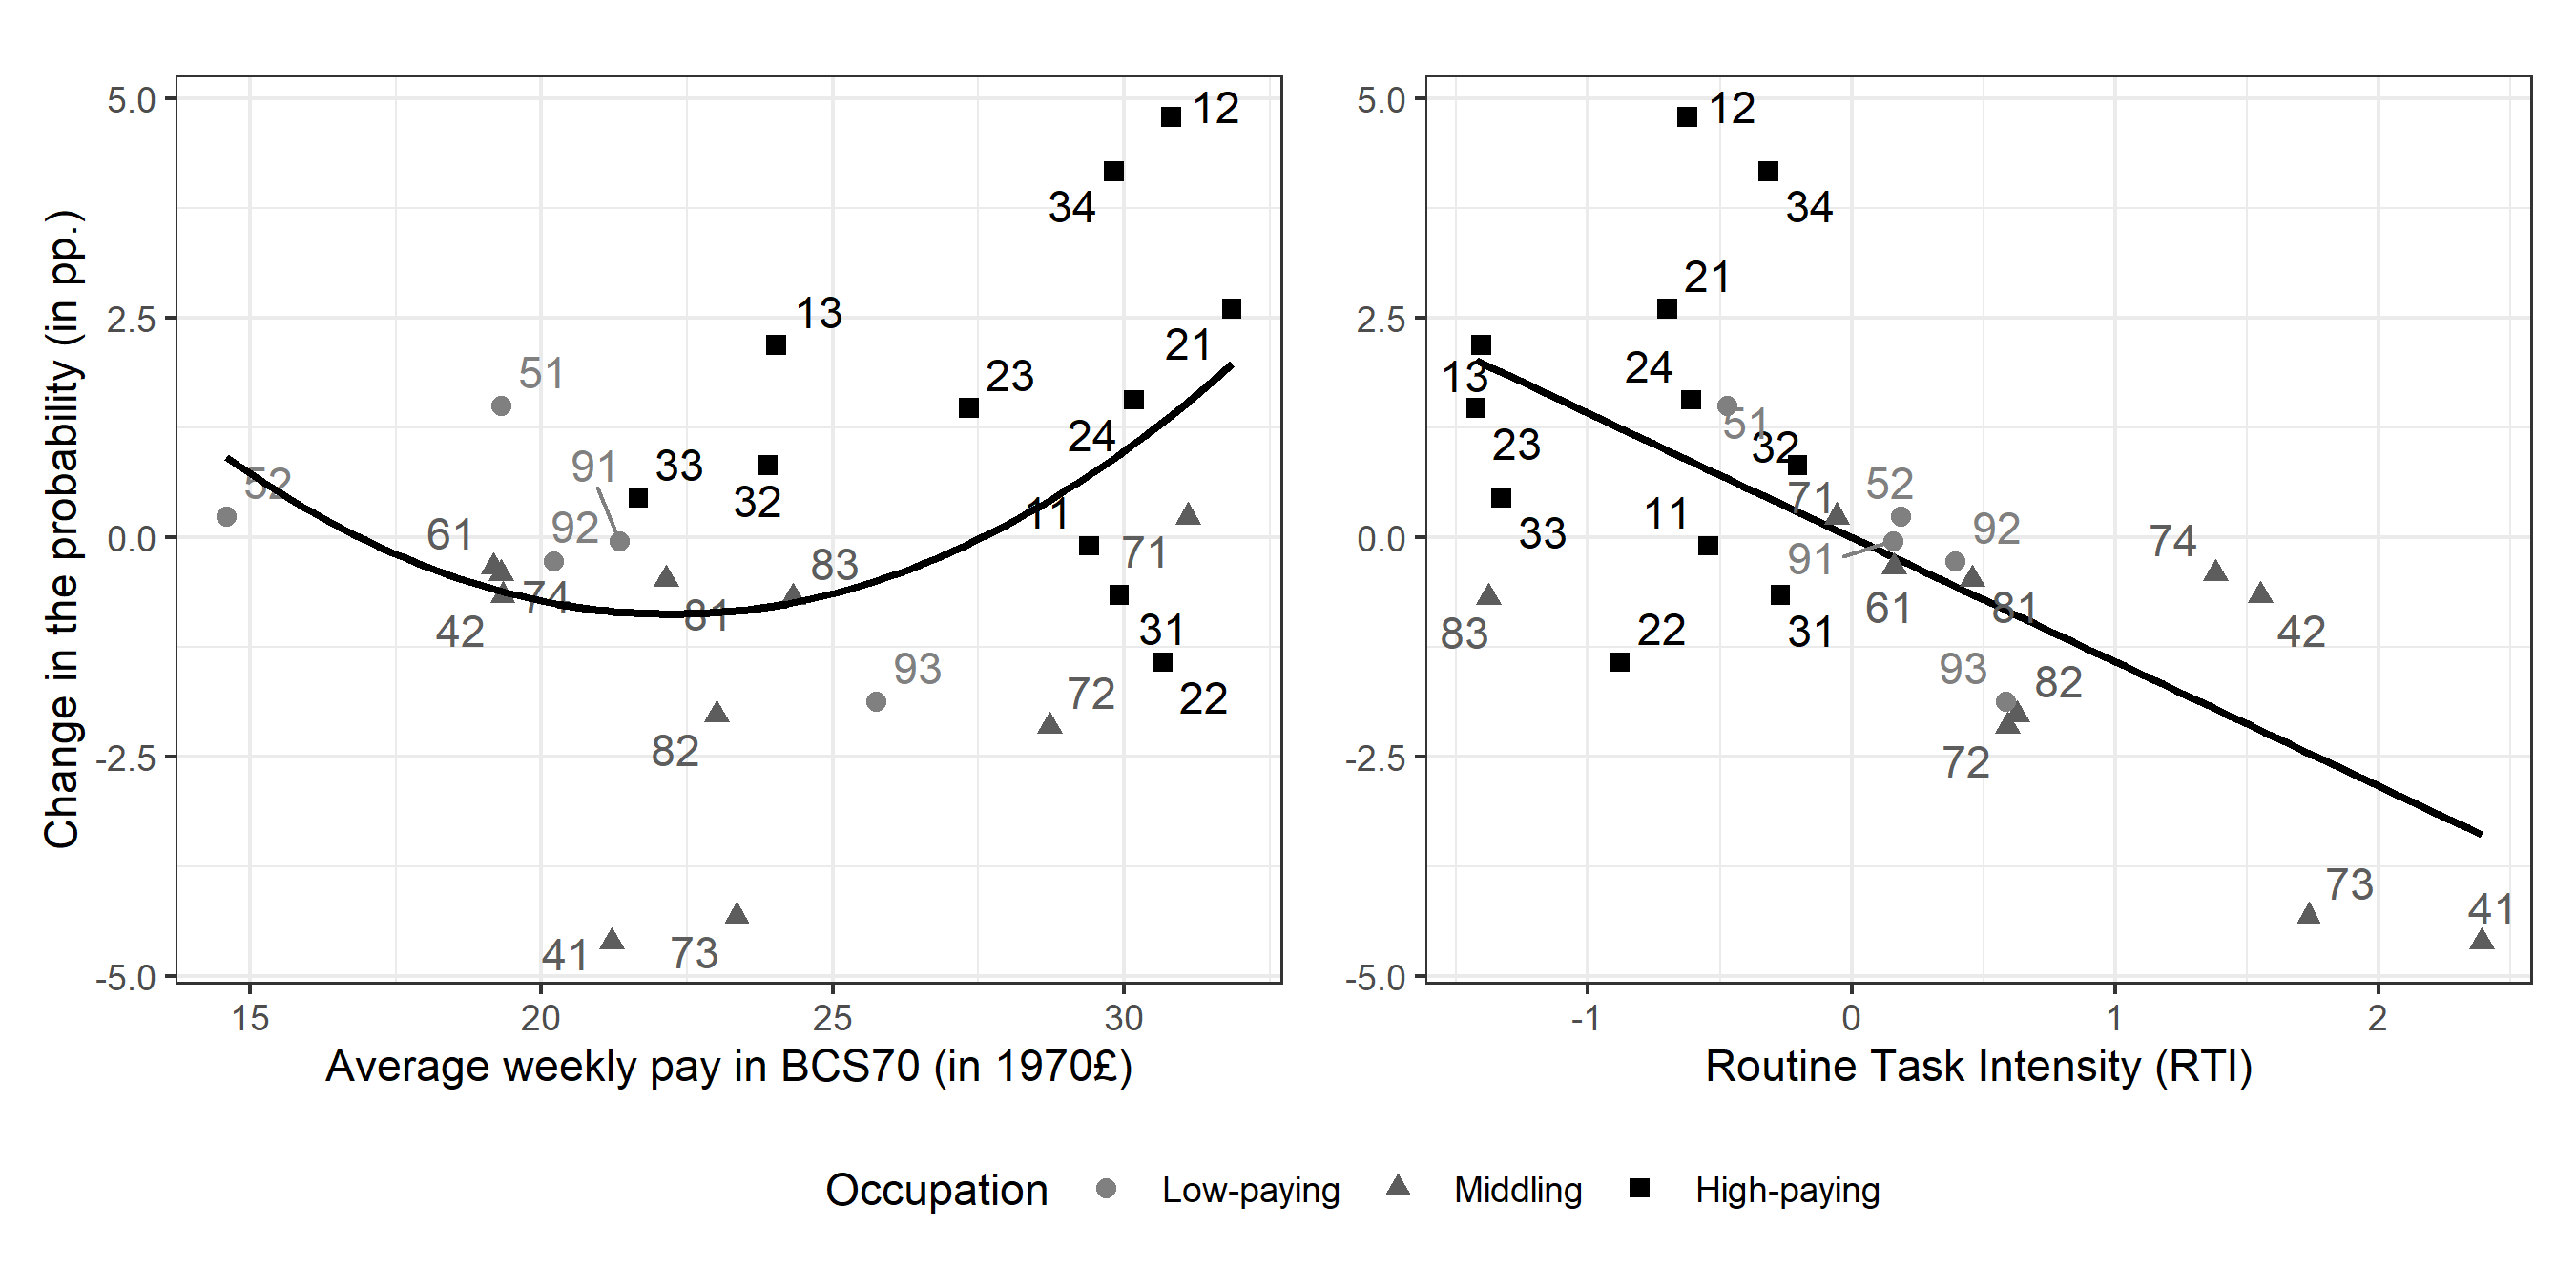
\includegraphics[width=\linewidth]{chap2/graphic/polarize-both-p1.png}
	\vspace{-3em}
	\justify\singlespacing\footnotesize{\textit{Notes:} The left-hand side panel of the figure presents the U-shaped relationship between the difference, expressed in percentage points, between the BCS70 and NCDS58 cohorts in terms of probability of being in each ISCO-88 occupation in the first period and the average weekly pay, expressed in 1970\pounds, in this occupation for the BCS70 cohort. The right-hand side panel shows the negative relationship between the difference, expressed in percentage points, between the BCS70 and NCDS58 cohorts in terms of probability of being in each ISCO-88 occupation in first period and the Routine Task Intensity (RTI) index from \cite{Mahutga2018Job}.}
\end{figure}
The right panel plots the change in the share of each occupation for young individuals against the RTI index provided by \cite{Mahutga2018Job}. The downward slopping line in Figure \ref{chap2-fig:polarize-both-p1} corresponds to the fitted curve implied by the data, and indicates that the change is negatively correlated with the degree of routinization. 

The various pieces of evidence in this section thus indicate that the strong polarization identified in cross-sectional data by previous work is also present when we focus on two specific cohorts. Routine intensity seems to be highly correlated with changes in the share of occupations, with low RTI ones having gained share and those with high RTI having lost it. Moreover, polarization appears whether we use the RTI index to categorize occupations or when we look at average weekly pay.

\subsection{Occupational dynamics} \label{chap2-dynamics}

While the literature on inter-generational mobility has traditionally focused on the outcomes of children when they are mature, we are interested in the occupational dynamics through which individuals reach a particular outcome. To illustrate why this is important, Table \ref{chap2-tab:proba-group4-cdt} reports the conditional probabilities of switching occupations between age 23/26 and age 42.\footnote{To understand why the probability of moving from out-of-work into a high-paying occupation is so high, recall that the former category includes those in education. Conditional probabilities in which we consider those in education as separate category, hence not included in out-of-work, are reported in the appendix, and display the expected (large) difference between those in education and the rest of those out-of-work; see Table \ref{chap2-tab:proba-group5-cdt-short}.}

\begin{table}[!tb]
    \centering
    \caption{Conditional probabilities of changing occupations}
    \label{chap2-tab:proba-group4-cdt}
    \begin{threeparttable}
        \small
        
\begin{tabular}{lrrrrrrrr}
\toprule
\multicolumn{1}{c}{} & \multicolumn{4}{c}{BCS70} & \multicolumn{4}{c}{NCDS58} \\
\cmidrule(l{3pt}r{3pt}){2-5} \cmidrule(l{3pt}r{3pt}){6-9}
Occupation & Out & Low & Mid & High & Out & Low & Mid & High\\
\midrule
Out-of-work & 33.8 & 25.3 & 14.5 & 26.4 & 27.4 & 24.7 & 20.7 & 27.3\\
Low-paying & 13.6 & 45.1 & 17.5 & 23.8 & 16.3 & 40.0 & 20.3 & 23.4\\
Middling & 10.5 & 13.8 & 44.9 & 30.8 & 10.4 & 15.4 & 43.4 & 30.8\\
High-paying & 8.3 & 8.2 & 11.0 & 72.6 & 8.5 & 8.1 & 12.3 & 71.2\\
\bottomrule
\end{tabular}

        \begin{tablenotes}[flushleft]
            \footnotesize{\item \textit{Notes}: This table shows the probability, expressed in percent, of being in each second-period occupation (columns) conditional on the first-period occupation (rows) for individuals in the NCDS58 and BCS70 cohorts.}
        \end{tablenotes}
    \end{threeparttable}
\end{table}

The table shows that there is a considerable degree of mobility across occupations over the individual's lifetime, i.e. of intra-generational mobility. Individuals who start their careers in low-paying and middling occupations have probabilities of staying there of around 40\% and a substantial likelihood of moving upwards. Notably, 30.8\% of those initially in middling occupations have a job in high-paying occupations by age 42 for both cohorts. In contrast, persistence is high for those who start in high-paying occupations, over 70\%. The transition probabilities are remarkably similar across cohorts, in particular those of moving into a high-paying occupation. The most significant differences come from the outcomes of those who start either out of work or in low-paying occupations. In both cases, those in the younger cohort face a lower probability of being in a middling occupation when mature (lower by 5.8 and 2.5 pp., respectively) which translates into higher odds of remaining in the occupation of origin. 

These figures indicate that the occupational outcomes of mature individuals depend both on their initial occupations and on the transitions across occupations, and raise the question of whether a reduction in the share of middling jobs can be a break to mobility. If mobility occurs partly through individuals progressing up the income ladder during their careers, the disappearance of middling jobs can have important consequences. On the one hand, a large proportion of those who are in high-paying occupations at age 42 start their careers in middling occupations. If fewer individuals are in such occupations when young, as indicated by Figure \ref{chap2-fig:stat-occ}, then there will be fewer individuals that can move into high-paying jobs. On the other, those who start in low-paying occupations have access to fewer middling jobs and hence are more likely to stay in their initial occupations. The importance of such changes for mobility will depend on the extent to which parental background matters for entry into each occupation and for the subsequent dynamics.
